\chapter{روش‌ها و مجموعه‌داده}
\section{بررسی آماری مجموعه داده}

در این پژوهش از مجموعه داده
\lr{PhysioNet}\cite{physionet_hssayeni2020intracranial,hssayeni2020computed}
استفاده شده است که شامل حاشیه‌نویسی برای وظیفه طبقه‌بندی و قطعه‌بندی است. این مجموعه داده  شامل مجموعه‌ای از سی‌تی‌اسکن‌های مغزی است که به صورت عمومی در دسترس است.
\begin{figure}[h]
\centering
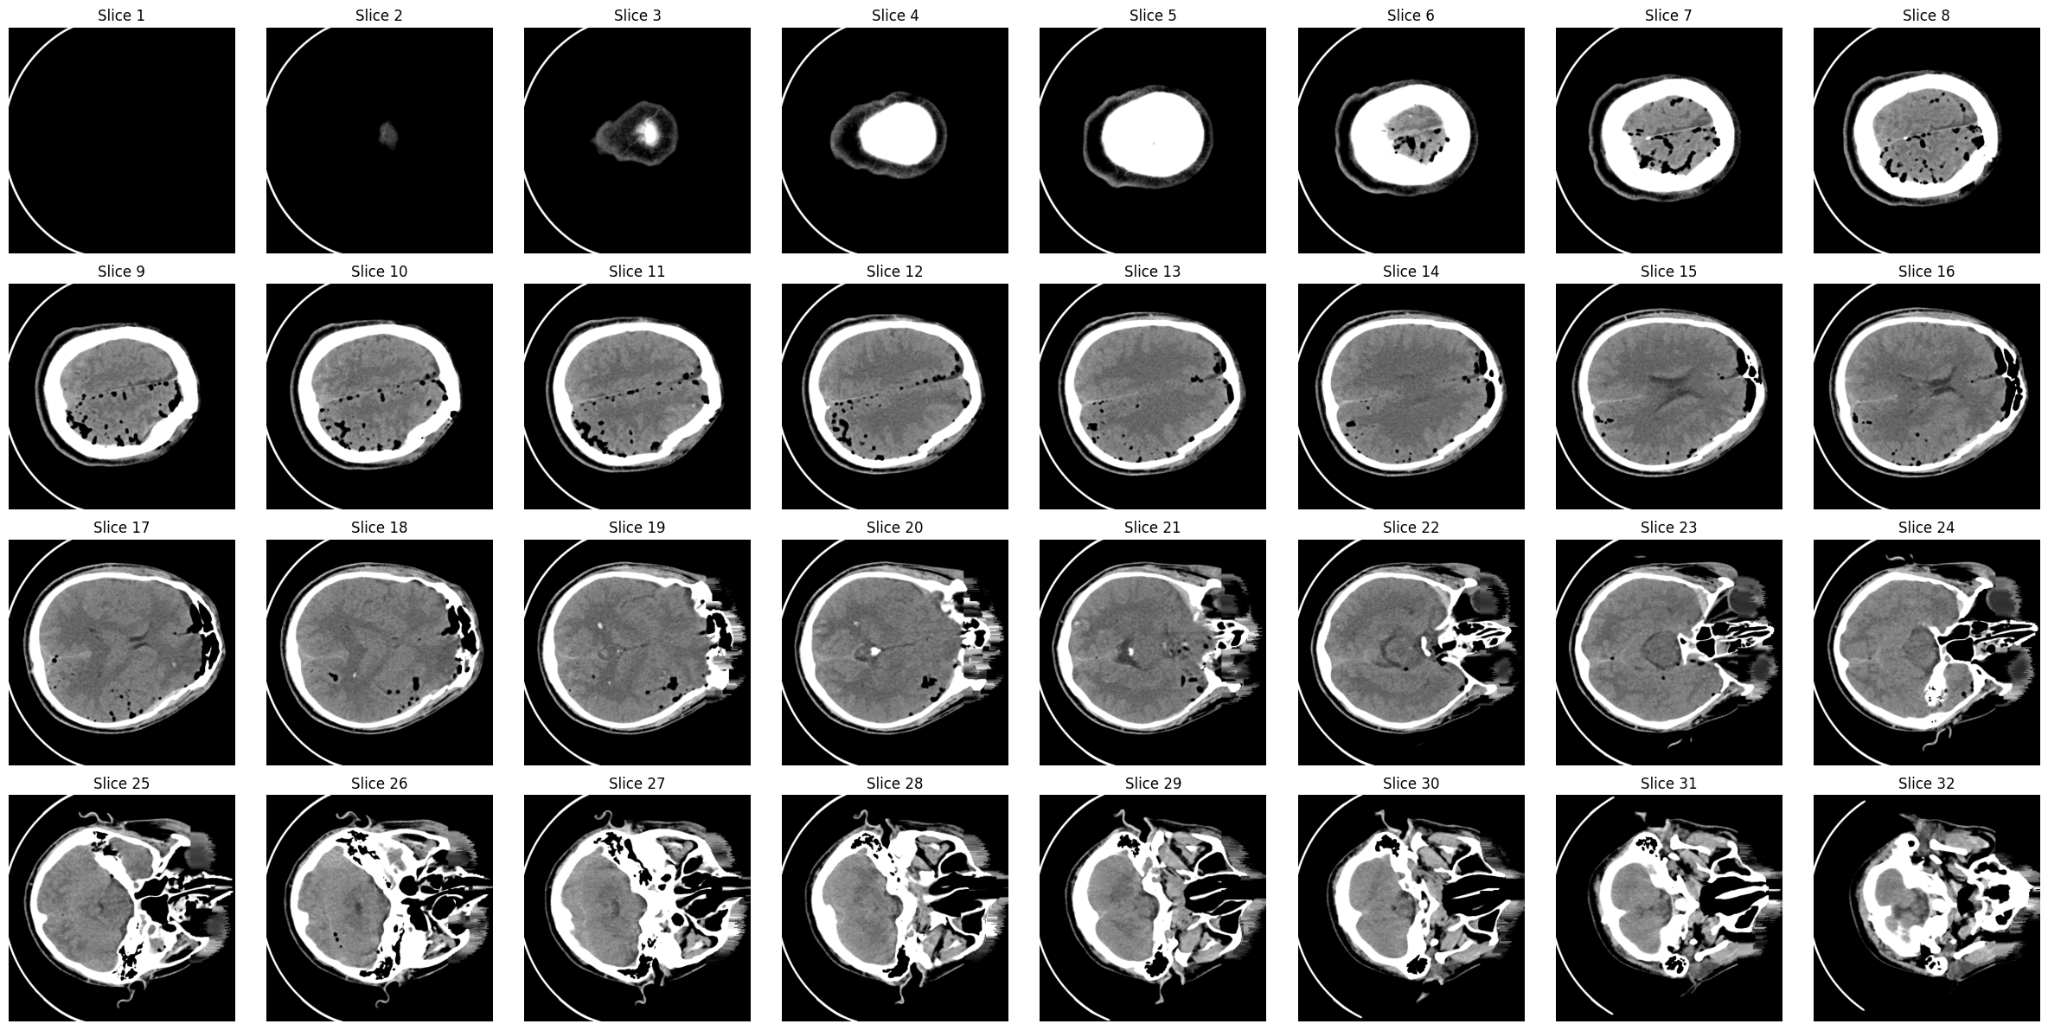
\includegraphics[width=1.0\linewidth]{Images/Chapter2/3d}
\caption{یک نمونه کامل از تصاویر سی‌تی‌اسکن}
\label{fig:ct2-3d}
\end{figure}


همانطور که در 
\autoref{fig:ct2-3d}
نمایش‌داده‌شده است، سی‌تی‌اسکن یک نوع تصویر سه‌بعدی است که از برش‌های دو بعدی تشکیل شده است. 
\autoref{fig:read-ct}
 نشان می‌دهد که
 با توجه به جهت بررسی برش‌های سی‌تی‌اسکن، این تصاویر به سه دسته 
 \lr{Axial}, \lr{Sagital} و \lr{Coronal}
 تقسیم می‌شوند.
\begin{figure}[h]
\centering
\includegraphics[width=1.0\linewidth]{"Images/Chapter2/read CT"}
\caption{خوانش‌های متفاوت از تصاویر سی‌تی‌اسکن
\cite{kaggleCTScansDICOM}}
\label{fig:read-ct}
\end{figure}
 
مجموعه‌داده 
\lr{PhysioNet}
 شامل 82 سی‌تی‌اسکن با برش‌‌های 
\lr{Axial}
است که بین فوریه و آگوست 2018 از بیمارستان آموزشی 
\lr{Al Hilla }
 در عراق جمع‌آوری شده است. این اسکن‌ها شامل طیف وسیعی از بیماران هستند که از یک روز تا 72 سال سن دارند و میانگین سن آنها 
 $27.8 \pm 19.5$
 سال است. تنوع سنی این مجموعه داده بر مقیاس، شکل جمجمه و بافت مغز در سی‌تی‌اسکن تأثیر می‌گذارد، عاملی که می‌تواند عملکرد مدل‌های یادگیری عمیق برای تشخیص و قطعه‌بندی خونریزی درون جمجمه‌ای را تحت تأثیر قرار دهد. توزیع جنسیت در ای نمجموعه‌داده به گونه‌ای است که 56\%  بیماران مرد و 44\% آنها زن هستند.
82 بیماری که در این مجموعه داده وجود دارد که 7 مورد از آنها طی قرایند حاشیه‌نویسی گم شده‌اند و از بین 75 بیمار موجود، 36 نفر دارای خونریزی درون‌جمجمه‌ای تشخیص داده شدند.
\autoref{fig:ch2-slice-number}
نمودار مروبط به تعداد برش‌های هر بیمار در این مجمموعه‌داده است؛ تصاویر سی‌تی‌اسکن موجود در این مجموعه داده،  به طور متوسط شامل 34 برش با ضخامت برش 5 میلی‌متر دارند و در مجموع 2814 برش در این مجموعه‌داده وجود دارد. 
\begin{figure}[h]
\centering
\includegraphics[width=1.0\linewidth]{"Images/Chapter2/Slice number"}
\caption{‌تعداد برش‌های بیماران بر اساس شناسه اختصاصی آنها}
\label{fig:ch2-slice-number}
\end{figure}

با این حال، این مجموعه داده به دلیل عدم توازن در سطح برش شناخته می‌شود، زیرا تنها 318 برش دارای خونریزی هستند در حالی که بقیه 2496 برش سالم هستند. در این مجموعه داده، 24 برش شامل زیرگروه
 \lr{IVH}،
  73 برش شامل زیرگروه
 \lr{CPH}، 
  18 برش شامل زیرگروه
 \lr{SDH}،
173 برش شامل زیرگروه
 \lr{EDH} 
 و 56 برش شامل زیرگروه 
 \lr{SDH}
هستند. با توجه به تفاوت شکل انواع زیرگروه‌های خونریزی و محل وقوع آنها، این ارقام نشان دهنده عدم وجود تعداد برش کافی برای بعضی از انواع زیرگروه‌های است.
در این مجموعه‌داده، برش‌های سی‌تی‌اسکن توسط دو پرتوشناس بررسی شده‌است و هر برش سی‌تی‌اسکن از نظر وجود خونریزی یا شکستگی توسط آنها بررسی و برچسب‌گذاری شده است. در ادامه سی‌تی‌اسکن‌های دو بیمار، به علت کیفیت ضعیف تصاویر و به توصیه پرتوشناس‌ها حذف شدند\cite{kyung2022improved}.

\autoref{fig: ch2-distribution}
نمودارهای توزیع بیمارمحور و برش‌محور مجموعه‌داده را نمایش می‌دهد؛ همانطور که از ‎\autoref{fig: ch2-patient distrbiution}‎ مشخص است در بررسی بیمار‌محور این مجموعه‌داده، عدم توازن دیده نمی‌شود اما در بررسی برش‌محور، همانطور که در ‎\autoref{fig: ch2-slice distribution}‎ 
مشخص است، عدم توازن شدیدی در تعداد برش‌های دارای خونریزی وجود دارد که این مسئله آموزش مدل‌های شبکه عصبی را با چالش مواجه می‌کند.
 \begin{figure}[ht]
		\centering % <-- added
		\begin{subfigure}{0.45\textwidth}
			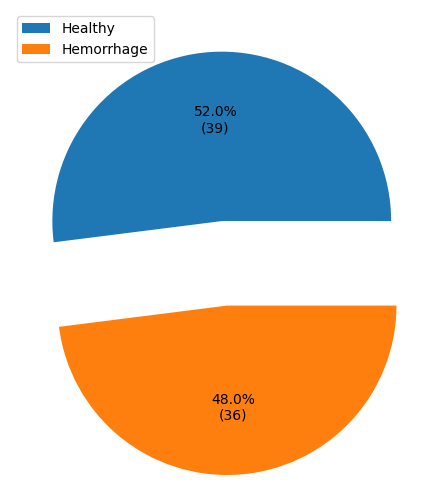
\includegraphics[width=\linewidth]{Images/Chapter2/patient distrbiution.png}
			\caption{}
			\label{fig: ch2-patient distrbiution}
		\end{subfigure}\hfil % <-- added
		\begin{subfigure}{0.45\textwidth}
			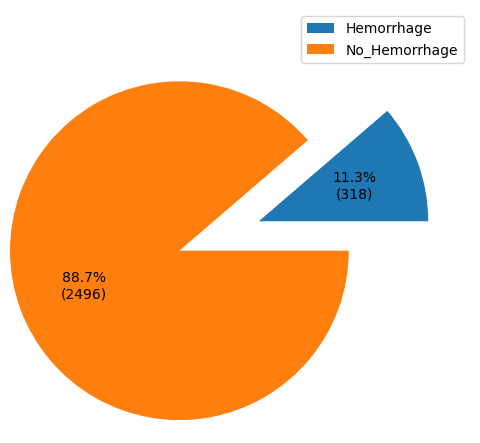
\includegraphics[width=\linewidth,]{Images/Chapter2/slice distribution.png}
			\caption{}
			\label{fig: ch2-slice distribution}
		\end{subfigure}
		\caption{توزیع بیماران و برش‌ها در مجموعه داده 
		\lr{PhysioNet}}
		\label{fig: ch2-distribution}
\end{figure} 

 علاوه بر وجود عدم توازن در حالت برش‌محور، عدم توازن شدیدی در قطعه‌بندی نواحی دارای خونریزی نسبت به نواحی سالم در برش‌های دارای خونریزی وجود دارد که به موجب آن در یک تصویر با ابعاد
$512\times512$،
به صورت میانگین نزدیک به 2000 پیکسل
\LTRfootnote{Pixel}
دارای خونریزی درون‌جمجمه‌ای وجود دارد که این مسئله آموزش مدل‌های شبکه عصبی را به منظور وظیفه قطعه‌بندی با چالش بسیار جدی مواجه می‌کند. 
\autoref{fig: ch2-slice hist}
نشان‌دهنده توزیع نرمال‌شده 
\LTRfootnote{Normalized}
مقدار پیکسل‌های برش‌های سالم و برش‌های دارای خونریزی می‌باشد، با توجه به
\autoref{fig: ch2-slice hist whole}، 
اکثر پیکسل‌های تصاویر مقداری نزدیک به 
$-1000$
و نقطه بیشینه محلی بعدی برای این نمودار توزیع، در نزدیک مقادیر 30 می‌باشد که این مقادیر به نسبت پیکسل‌ها با مقادیر نزدیک به 
$-1000$
خیلی کمتر می‌باشد.


 \begin{figure}[ht]
		\centering % <-- added
		\begin{subfigure}{0.45\textwidth}
			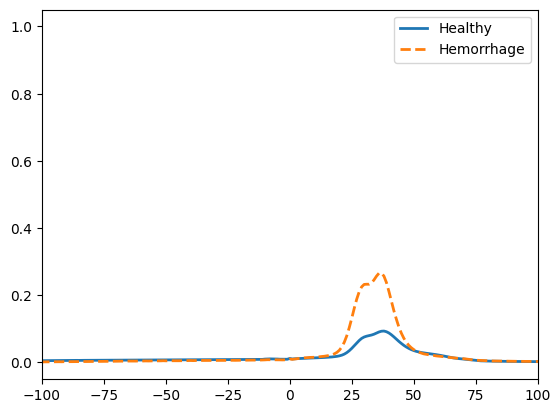
\includegraphics[width=\linewidth]{Images/Chapter2/Pixel histogram.png}
			\caption{}
			\label{fig: ch2-slice hist whole}
		\end{subfigure}\hfil % <-- added
		\begin{subfigure}{0.45\textwidth}
			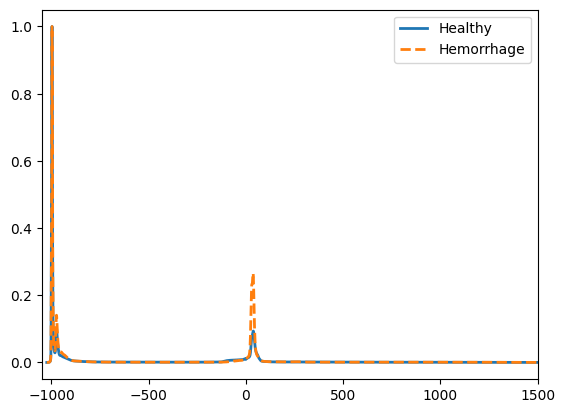
\includegraphics[width=\linewidth,]{Images/Chapter2/Pixel histogram lim.png}
			\caption{}
			\label{fig: ch2-slice hist lim}
		\end{subfigure}
		\caption{توزیع پیکسلی برش‌ها برای برش‌های داداری خونریزی در مقال برش‌های سالم}
		\label{fig: ch2-slice hist}
\end{figure} 

\autoref{fig:ch2-pixel-hist-ich-vs-healthy}
نمایش‌دهنده توزیع پیکسل‌های دارای خونریزی و تمام پیکسل‌های تصاویر رادیوگرافی می‌باشد که در محدوده بین 
$-100$
تا 
$100$
واقع شده است و نسبت به مقادیر همین بازه نرمال گشته است. همانطور که از این دو نمودار مشخص است، مقادیر مربوط به ضایعه خونریزی،‌مقادر کمی از مقادیر بقیه بافت‌های مغز روشن‌تر است اما همپوشانی این دو نمودار نشان می‌دهد که تشخیص خونریزی درون‌جمجمه‌ای تنها با استفاده از مقدار پیکسلی آن بسیار دشوار می‌باشد و نیاز هست تا از شبکه‌هایی استفاده شود تا به اشکال موجود در تصویر نیز حساسیت داشته باشند.


\begin{figure}[h]
\centering
\includegraphics[width=1.0\linewidth]{"Images/Chapter2/pixel hist ich vs healthy"}
\caption{توزیع نرمال‌شده پیکسل‌های دارای خونریزی درمقابل تمام پیکسل‌های تصاویر}
\label{fig:ch2-pixel-hist-ich-vs-healthy}
\end{figure}


\autoref{fig:ch2-slice-number}
توزیع خونریزی درون‌جمجمه‌ای را بر اساس شماره برش در تصویر سی‌تی‌اسکن نشان می‌دهد که بر اساس آن مشخص است به ازای بعضی از شماره برش‌ها، خونریزی درون‌جمجمه‌ای وجود ندارد و این برش‌ها از اهمیت کمتری برای مدل‌های یادگیری ماشین برخوردار هستند.

\begin{figure}[h]
\centering
\includegraphics[width=1.0\linewidth]{"Images/Chapter2/slice hist"}
\caption{توزیع خونریزی بر اساس برش‌ها}
\label{fig:ch2-slice-hist}
\end{figure}


باتوجه به مطالبی که دی این بخش مطرح شد،‌می‌توان نتیجه‌ گرفت که مجموعه داده
 \lr{PhysioNet}،
به عنوان تنها مجموعه‌داده عمومی قطعه‌بندی خونریزی درون‌جمجمه‌ای، می‌تواند یک مجموعه‌داده معیار برای بررسی عملکرد مدل‌های پردازش تصویر باشد. 


\section{پیش‌پردازش\protect\LTRfootnote{Pre-process}}

در تصاویر پرتونگاری سی‌تی‌اسکن، از اشعه ایکس
\LTRfootnote{X-Ray}
 به منظور ثبت تصویر اندام درونی بدن استفاده می‌شود. در این روش،‌یک کاتد
 \LTRfootnote{Cathode}
را برانگیخته می‌کنند تا الکترون‌های
 \LTRfootnote{Electron}
 پرانرژی را آزاد ‌کند. با آزاد شدن الکترون‌ها، انرژی به صورت اشعه ایکس آزاد می‌شود و اشعه ایکس از بافت‌ها عبور کرده و به آشکارساز در سمت دیگر برخورد می‌کند. هرچه بافت متراکم‌تر باشد، اشعه ایکس بیشتری را جذب می‌کند؛ مثلا باقت استخوانی به علت تراکم بالا،‌ اشعه ایکس بیشتری جذب می‌کند و در نتیجه آن اشعه کمتری به آشکارساز می‌رسد که موجب سفید شدن آن قسمت از تصویر خواهد شد اما این مسئله درمورد هوا برعکس است
 \cite{kaggleCTScansDICOM}.
در مقایسه با تصویر اشعه ایکس ساده، سی‌تی‌اسکن دارای تفکیک‌پذیری بیشتر است و هیچ هم‌پوشانی در ساختارها وجود ندارد.
دستگاه‌های سی‌تی‌اسکن که از کالیبراسیون
\LTRfootnote{Calibration}
 درستی برخوردار باشند، تصاویر خود را طبق یکای 
 \lr{Hounsfield}
ثبت می‌کنند. این یکا به پرتونگارها و محققین اجازه می‌دهد تا بتوانند با آستانه گذاری مناسب، جزییات بافت هدف خود را در تصویر رویت‌پذیرتر کنند. تصاویر سی‌تی‌اسکن به صورت معمول بر اساس یکای
\lr{Hounsfield}
 مقادیر پیکسلی بین $-1024$ تا 3000 را دارا می‌باشند.

\autoref{fig:ch2-hu}
نشان‌دهنده مقدار پیکسلی است که هر بافت در تصویر سی‌تی‌اسکن از خود نشان می‌دهد. پروتونگارها،‌ پزشک‌ها و محققین برای اینکه بتوانند یک بیماری خاص را مورد بررسی قرار بدهند، برش‌های تصاویر را در بازه‌های خاصی از یکای
\lr{Hounsfield}
مورد بررسی قرار می‌دهند که به این نوع از پیش‌پردازش تصاویر سی‌تی‌اسکن،‌پنجره‌گذاری
\LTRfootnote{Windowing}
می‌گویند. 
\begin{figure}[h]
\centering
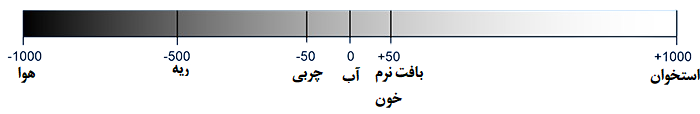
\includegraphics[width=1.0\linewidth]{Images/Chapter2/HU}
\caption{اثر بافت‌های متفاوت در یکای
 \lr{Hounsfield}
 \cite{kaggleCTScansDICOM}}
\label{fig:ch2-hu}
\end{figure}

در روش پنجره‌گذاری، دو مقدار مرکز پنجره
\lr{(WC)}
و پهنای پنجره
\lr{(WW)}
بازه هدف را در تصویر مشخص می‌کند و به موجب آن هر پیکسل که مقدار آن از حداقل بازه کمتر باشد، مقدارش برابر با حداقل بازه می‌شود و هر پیکسل که مقدارش از حداکثر بازه بیشتر باشد، مقدارش برابر حداکثر بازه می‌شود. ‎
\autoref{code:ch2-windowing}
روش اعمال پنجره‌گذاری روی تصاویر را نمایش می‌دهد که در آن 
\lr{Normalize}
به منظور انتقال مقادیر تصویر بعد از پنجره‌گذاری بین 0 و 1 است و 
\lr{Threshold}
تابعی است که در اثر آن مقادیر کمتر از حداقل بازه هدف به مقدار خداقل تغییر پیدا می‌کنند و مقادیری بیشتر از حداکثر بازه به مقدار حداکثر تبدیل می‌شوند.   
\begin{latin}
\begin{equation}
\text{Processed Image} = \text{Normalize}(\text{Threshold}(\text{Image}, WC-\frac{WW}{2},WC+\frac{WW}{2})) 
\end{equation}
\label{code:ch2-windowing}
\end{latin}

پرتونگار‌ها مقادیر مشخصی را برای شناسایی انواع مختلف اندام در تصاویر سی‌تی‌اسکن تعیین کرده‌اند به عنوان مثال، در مجموعه‌داده
\lr{‌PhysioNet}،
پردازش تصویر اصلی به‌ازای مرکز پنجره 40 و پهنای پنجره 120، پنجره مغز استخراج می‌شود و به‌ازای مرکز پنجره 700 و پهنای پنجره 3200،‌ پنجره استخوان استخراج می‌شود.
\autoref{fig:ch2-windowed-ct-sample}
اثر پنجره‌گذاری را بر یک نمونه برش سی‌تی‌اسکن نشان می‌دهد. همانطور که از این
\autoref{fig:ch2-before-processing}
 مشخص است، تصویر قبل از پیش‌پردازش جزییات خاصی را به ما نشان نمی‌دهد و اگر این تصویر را بدون نرمال کردن برای آموزش شبکه‌عصبی استفاده کنیم، باعث می‌شود که لایه‌های ابتدایی شبکه مقادیر خیلی بزرگی را ایجاد کنند و در نتیجه عملکرد مدل کاهش پیدا بکند و اگر این تصویر را نرمال کنیم، به علت بازه بسیار زیاد یکای 
\lr{Hounsfield}
تفکیک‌پذیری مقادیر تصویر به شدت کاهش پیدا می‌کند. در ادامه
\autoref{fig:ch2-brain-window}, \autoref{fig:ch2-bone-window} و \autoref{fig:ch2-subdural-window}
اثر سه پنجره مرسوم مغز، استخوان و سابدورال را مشاهده می‌کنیم که هرکدام تفکیک‌پذیری بافت هدف خود را افزایش داده‌اند و در پنجره مغز و سابدورال، محل خونریزی به وضوح مشخص است.
\autoref{fig:ch2-selected-window}
 پنجره انتخابی را نشان می‌دهد که براساس محدوده موجود در  
\autoref{fig:ch2-pixel-hist-ich-vs-healthy}
انتخاب شده‌است و در نتیجه آن، محل خونریزی بروز بیشتری پیدا کرده است. در ادامه این پژوهش،‌ پنجره مغز به عنوان پنجره اصلی آموزش و ارزیابی مدل‌ها درنظر گرفته شده است.




\begin{figure}[h!]
    \centering % <-- added
    \begin{subfigure}{0.33\textwidth}
      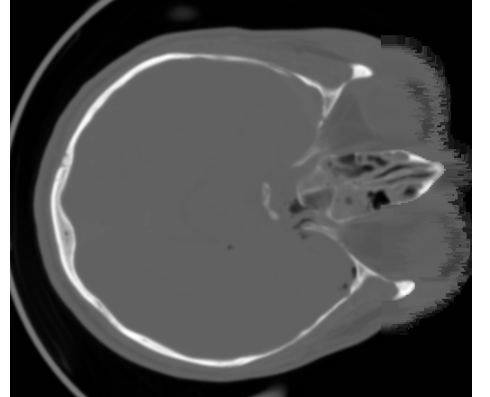
\includegraphics[width=\linewidth]{Images/chapter2/before_processing_no_caption.png}
      \caption{قبل از پردازش}
      \label{fig:ch2-before-processing}
    \end{subfigure}\hfil % <-- 
    \begin{subfigure}{0.33\textwidth}
      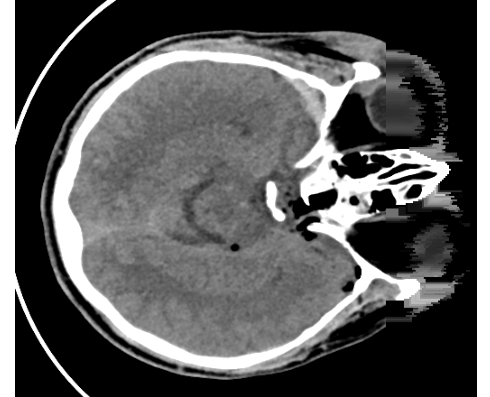
\includegraphics[width=\linewidth]{Images/chapter2/brain_window_no_caption.png}
      \caption{پنجره مغز}
      \label{fig:ch2-brain-window}
    \end{subfigure}\hfil % <-- 
    \begin{subfigure}{0.33\textwidth}
      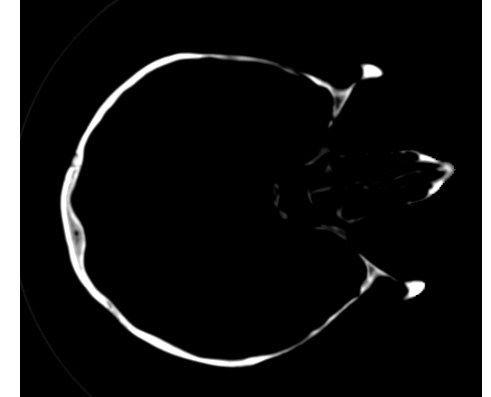
\includegraphics[width=\linewidth]{Images/chapter2/bone_window_no_caption.png}
      \caption{پنجره استخوان}
      \label{fig:ch2-bone-window}
    \end{subfigure}\hfil % <-- 
    \begin{subfigure}{0.33\textwidth}
      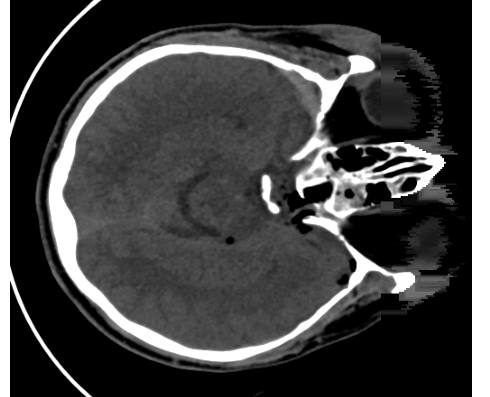
\includegraphics[width=\linewidth]{Images/chapter2/subdural_window_no_caption.png}
      \caption{پنجره ساب‌دورال}
      \label{fig:ch2-subdural-window}
    \end{subfigure}\hfil % <-- 
    \begin{subfigure}{0.33\textwidth}
      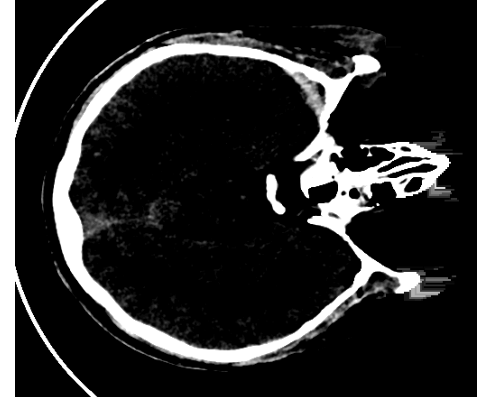
\includegraphics[width=\linewidth]{Images/chapter2/selected_window_no_caption.png}
      \caption{پنجره انتخابی}
      \label{fig:ch2-selected-window}
    \end{subfigure}\hfil % <-- 
    \begin{subfigure}{0.33\textwidth}
      
\includegraphics[width=\linewidth]{Images/chapter2/bleed_location_no_caption.png}
      \caption{محل خونریزی}
      \label{fig:ch2-bleed-location}
    \end{subfigure}
\caption{تاثیر اثر پنجره‌گذاری در نمایش خونریزی در یک برش از سی‌تی‌اسکن}
\label{fig:ch2-windowed-ct-sample}
\end{figure}

\section{روش پردازش تصاویر}
شبکه‌های عصبی عمیق به عنوان یکی از روش‌های محبوب در حوزه‌ی یادگیری ماشین شناخته می‌شوند. این شبکه‌ها از ساختارهایی شبیه به مغز انسان تشکیل شده‌اند که شامل تعدادی نورون \LTRfootnote{Neuron} مصنوعی هستند و قادرند با استفاده از داده‌های ورودی، الگوها و روابط پیچیده را بیاموزند. یادگیری عمیق، شاخه‌ای از شبکه‌های عصبی است که با افزایش تعداد لایه‌های مخفی در شبکه، امکان پردازش و تحلیل داده‌های بسیار پیچیده و بزرگ را فراهم می‌کند.
در این پژوهش، روش اصلی مورد استفاده برای پردازش کامپیوتری تصاویر، یادگیری عمیق است.
\subsection{یادگیری عمیق و اصول اولیه}
یادگیری عمیق یکی از شاخه‌های مهم یادگیری ماشین است که به دلیل توانایی‌های خود در پردازش، تحلیل و الگویابی در داده‌های پیچیده، به‌ویژه در حوزه‌ی پزشکی، به طور گسترده‌ای مورد استفاده قرار گرفته است. در این بخش، به بررسی اصول پایه‌ای یادگیری عمیق در پردازش تصویر پرداخته شده است.

\subsubsection{ساختار نورون}
شبکه‌های عصبی مصنوعی از تعدادی واحد پردازشی به نام نورون تشکیل شده‌اند. هر نورون چندین ورودی \(x_1, x_2, \ldots, x_n\) دریافت می‌کند که هر یک با وزن‌های \(w_1, w_2, \ldots, w_n\) متناظر ضرب می‌شوند. سپس، مجموع وزن‌دار ورودی‌ها به اضافه‌ی یک بایاس \(b\) مطابق با \autoref{eq:sum_weights} محاسبه شده و از طریق یک تابع فعال‌سازی \(\phi\) به خروجی تبدیل می‌شود، که رابطه آن در \autoref{eq:activation} مشخص شده است.

\begin{latin}
\begin{equation}
\label{eq:sum_weights}
z = \sum_{i=1}^{n} w_i x_i + b
\end{equation}
\end{latin}

\begin{latin}
\begin{equation}
\label{eq:activation}
a = \phi(z)
\end{equation}
\end{latin}

توابع فعال‌سازی به منظور ایجاد خاصیت غیرخطی در نورون‌ها استفاده‌می‌شوند تا با استفاده از شبکه عصبی عمیق،‌ بتوانیم توابع غیرخطی را تخمین بزنیم. دو تابع فعال‌سازی رایج عبارتند از
 \lr{ReLU}\LTRfootnote{Rectified Linear Unit} و
 \lr{Sigmoid}\LTRfootnote{Sigmoid}.
  رابطه تابع
   \lr{ReLU}
    در
     \autoref{eq:relu}
      مشخص شده است و رابطه تابع 
      \lr{Sigmoid}، 
      در
      \autoref{eq:sigmoid}
      مشخص شده است.

\begin{latin}
\begin{equation}
\label{eq:relu}
\phi(z) = \max(0, z)
\end{equation}
\end{latin}

و تابع سیگموید نیز به صورت زیر تعریف می‌شود:

\begin{latin}
\begin{equation}
\label{eq:sigmoid}
\phi(z) = \frac{1}{1 + e^{-z}}
\end{equation}
\end{latin}


\subsubsection{لایه‌های پنهان}
شبکه‌های عصبی عمیق از چندین لایه‌ی پنهان تشکیل شده‌اند که هر کدام از تعداد زیادی نورون مشابه نورون‌های توصیف‌شده در بخش قبلی تشکیل شده‌اند. خروجی هر نورون در یک لایه به عنوان ورودی برای نورون‌های لایه‌ی بعدی استفاده می‌شود. این ساختار چندلایه به شبکه امکان می‌دهد تا ویژگی‌های پیچیده و  رفتار غیرخطی را از داده‌های ورودی استخراج کند.
\autoref{fig:ch2-neuron}
نمایش نحوه مدلسازی یک نورون را با استفاده از 
\autoref{eq:sum_weights} و \autoref{eq:activation}
نشان می‌دهد و در ادامه نحوه عملکرد لایه‌های پنهان در شبیه‌سازی ارتباط بین نرون‌ها را نشان می‌دهد. 
\begin{figure}[h]
\centering
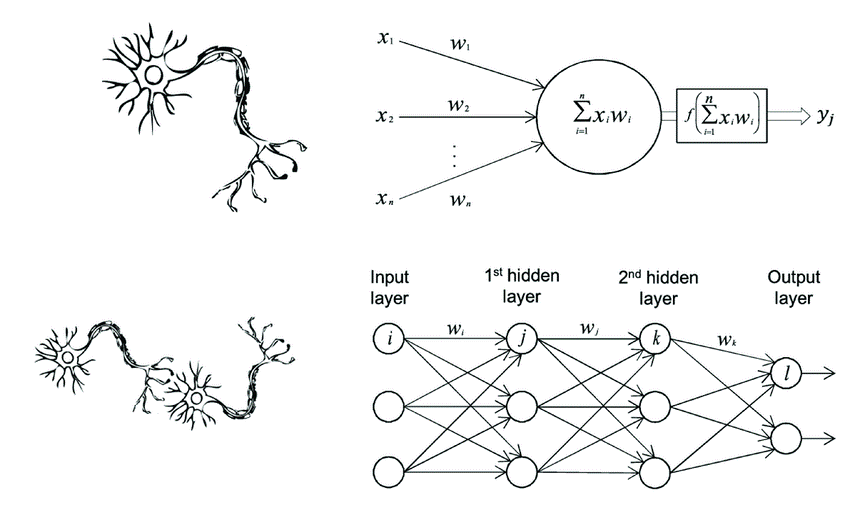
\includegraphics[width=1.0\linewidth]{Images/Chapter2/neuron}
\caption{مدلسازی یک نورون عصبی توسط رابطه ریاضی و ارتباط بین نرون‌ها با استفاده از لایه‌های پنهان}
\label{fig:ch2-neuron}
\end{figure}


\subsubsection{تابع خطا و پس‌انتشار
\protect\LTRfootnote{backpropagation}}
تابع خطا
 \LTRfootnote{Loss Function}
  نقش کلیدی در آموزش شبکه‌های عصبی دارد. این تابع تفاوت بین خروجی پیش‌بینی‌شده
  \lr{ \(y_{\text{pred}}\)}
   و خروجی واقعی
    \lr{\(y_{\text{true}}\)}
     را محاسبه می‌کند. یکی از رایج‌ترین توابع خطا، خطای 
  \lr{Binary Cross Entropy(BCE)}
   است که طبق 
   \autoref{eq:bce_loss}
   برای مسائل دسته‌بندی دوتایی استفاده می‌شود.

\begin{latin}
\begin{equation}
\label{eq:bce_loss}
L(\mathbf{y}_{\text{true}}, \mathbf{y}_{\text{pred}}) = -\frac{1}{m} \sum_{i=1}^{m} \left[ y_{\text{true}}^{(i)} \log(y_{\text{pred}}^{(i)}) + (1 - y_{\text{true}}^{(i)}) \log(1 - y_{\text{pred}}^{(i)}) \right]
\end{equation}
\end{latin}


هدف از آموزش شبکه، کمینه‌سازی این تابع خطا است که با استفاده از الگوریتم پس‌انتشار انجام می‌شود. در این روش، گرادیان
\LTRfootnote{Gradient}
 تابع خطا نسبت به هر وزن \(w_i\) طبق \autoref{eq:gradient} و قانون مشتقات زنجیره‌ای، محاسبه شده و سپس وزن‌ها با استفاده از قانون گرادیان کاهشی مطابق \autoref{eq:weight_update} به‌روزرسانی می‌شوند:

\begin{latin}
\begin{equation}
\label{eq:gradient}
\frac{\partial L}{\partial w_i}
\end{equation}
\end{latin}

\begin{latin}
\begin{equation}
\label{eq:weight_update}
w_{i+1} \leftarrow w_i - \eta \frac{\partial L}{\partial w_i}
\end{equation}
\end{latin}

\subsubsection{لایه‌های پرسپترون
\protect\LTRfootnote{Perceptron}
 چندلایه}
لایه‌های پرسپترون چندلایه
 \lr{(MLP)} 
 یکی از ساده‌ترین و پایه‌ای‌ترین ساختارها در شبکه‌های عصبی هستند. این لایه‌ها از تعدادی نورون تشکیل شده‌اند که به صورت کامل به یکدیگر متصل هستند؛ به بیان دیگر هر نورون در یک لایه به تمامی نورون‌های لایه‌ی قبلی متصل می‌شود و اطلاعات را به لایه‌ی بعدی منتقل می‌کند. خروجی هر لایه \(a^{[l]}\) از ترکیب خطی ورودی‌ها و اعمال تابع فعال‌سازی طبق \autoref{eq:mlp_output} به دست می‌آید:

\begin{latin}
\begin{equation}
\label{eq:mlp_output}
a^{[l]} = \phi(W^{[l]} a^{[l-1]} + b^{[l]})
\end{equation}
\end{latin}

\subsubsection{شبکه عصبی پیچشی
\protect\LTRfootnote{Convolutional Neural Network}}
برای بهبود عملکرد شبکه‌های عصبی در پردازش تصاویر، از لایه‌های شبکه عصبی پیچشی
\lr{(CNN)} 
استفاده می‌شود. در این لایه‌ها، عملیات کانولوشن به جای ضرب ماتریسی بین ورودی و وزن‌ها طبق \autoref{eq:convolution} انجام می‌شود. این عملیات برای هر ناحیه کوچک از تصویر با استفاده از یک فیلتر \(k\) صورت می‌گیرد.

\begin{latin}
\begin{equation}
\label{eq:convolution}
z_{i,j} = (X * k)_{i,j} = \sum_{m}\sum_{n} X_{i+m,j+n} \cdot k_{m,n}
\end{equation}
\end{latin}

خروجی این عملیات، نقشه ویژگی
\lr{Feature Map}
 است که به لایه بعدی منتقل می‌شود. با عبور یک تصویر از لایه‌های یک شبکه عصبی پیچشی، بین پیکسل‌های کنارهم در تصویر، یک رابطه برقرار می‌شود که درنتیجه آن، نقشه ویژگی استخراج شده برای هر پیکسل،‌ به وضعت پیکسل‌های اطرافش بستگی دارد و هرچه از پیکسل مبدا دور شویم، اثر آن در نقشه ویژگی کاهش پیدا می‌کند.
 
 




\subsubsection{بهینه‌سازها و الگوریتم 
\lr{Adam}
}

بهینه‌سازی یکی از مهم‌ترین اجزا در آموزش شبکه‌های عصبی هستند که هدف آنها به‌روزرسانی وزن‌ها به گونه‌ای است که تابع خطا به حداقل مقدار خود برسد. برای این منظور، از الگوریتم‌هایی استفاده می‌شود که بهینه‌ساز نامیده می‌شوند. 
یکی از رایج‌ترین بهینه‌سازها، الگوریتم گرادیان کاهشی است که در آن وزن‌ها در جهت منفی گرادیان تابع خطا به‌روزرسانی می‌شوند، هرابطه گرادیات کاهشی در \autoref{eq:weight_update} نشان داده شده است. 
 یکی دیگر از بهینه‌سازهای پیشرفته و کارآمد، بهینه‌ساز 
\lr{Adam}
 است. این بهینه‌ساز از ترکیب دو روش
\lr{Momentum}
 و
\lr{RMSProp}
 بهره می‌برد 
 \cite{towardsdatascienceUnderstandingDeep,mediumMomentumRMSpropAdam}.
  به‌روزرسانی وزن‌ها در \lr{Adam} با استفاده از روابط در 
  \autoref{eq:adam}
  انجام می‌شود.

\begin{latin}
\begin{equation}
\label{eq:adam}
\begin{aligned}
m_t &= \beta_1 m_{t-1} + (1 - \beta_1) \nabla L(\theta_t)\\
v_t &= \beta_2 v_{t-1} + (1 - \beta_2) (\nabla L(\theta_t))^2\\
\theta_{t+1} &= \theta_t - \eta \frac{\hat{m}_t}{\sqrt{\hat{v}_t} + \epsilon}
\end{aligned}
\end{equation}
\end{latin}


در این معادلات، \(m_t\) و \(v_t\) به ترتیب تخمین میانگین حرکت‌دار گرادیان و میانگین حرکت‌دار مربعات گرادیان در زمان \(t\) هستند، و \(\beta_1\) و \(\beta_2\) ضرایب مربوط به این میانگین‌ها هستند. \(\eta\) نرخ یادگیری و \(\epsilon\) یک مقدار بسیار کوچک برای جلوگیری از تقسیم بر صفر است. 
\lr{Adam} به دلیل توانایی خود در تنظیم نرخ یادگیری برای هر پارامتر به‌طور خودکار، به یکی از پرکاربردترین بهینه‌سازها در آموزش شبکه‌های عصبی عمیق تبدیل شده است. 